%%% FIGURES %%%

\begin{figure}
\centering
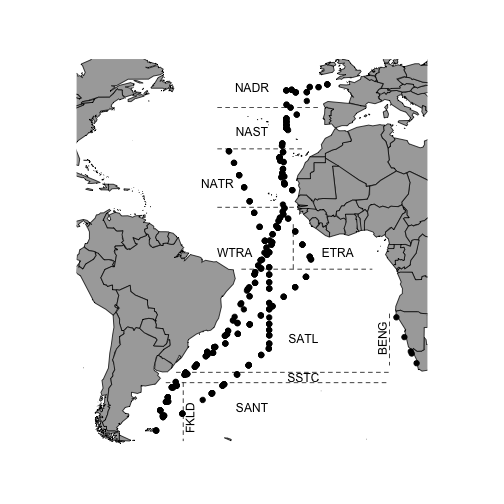
\includegraphics[trim = 30mm 20mm 25mm 20mm, clip, width=0.5\linewidth]{./Chp2-Pre/amt_mapFINAL2.png}
\caption[Scheme]{\small {The AMT subset of 410 samples used in this study. The dashed lines represent the simplified limits of the Longhurst (2006) ecological provinces.}}
\label{Map}
\end{figure}

\begin{figure}
\centering
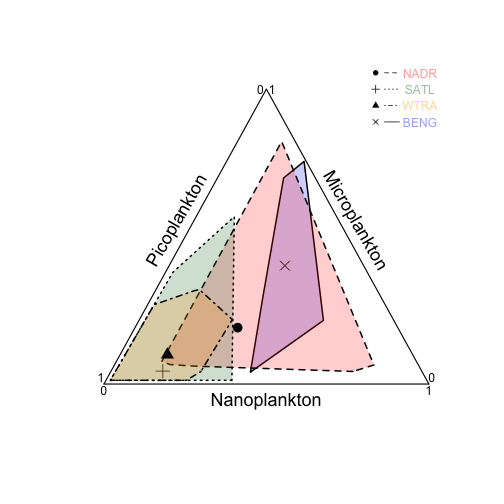
\includegraphics[trim = 20mm 30mm 20mm 20mm, clip, width=0.6\linewidth]{./Chp2-Pre/amt_4RegionsTriSizeFrac4.png}
\caption[Scheme]{\small {Phytoplankton community size structure of four ecological provinces in the Atlantic Ocean. The contours correspond to the convex hull of the size-fraction distribution of each province. The symbols indicate the corresponding mean values.}}
\label{RegSizeFrac}
\end{figure}

\begin{figure}
\centering
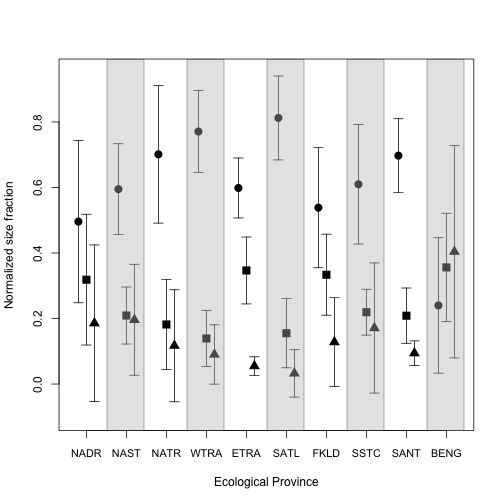
\includegraphics[trim = 0mm 0mm 0mm 0mm, clip, width=0.9\linewidth]{./Chp2-Pre/amt_MeanSDProvinces.png}
\caption[Scheme]{\small {Relative mean abundances ($\pm$sd) of three phytoplankton size fractions of ten ecological provinces of the Atlantic Ocean. The symbols indicate the mean values of the normalized size fractions: picoplankton (\ding{108}), nanoplankton(\ding{110}) and microplankton (\ding{115}).}}
\label{means}
\end{figure}

\begin{figure}
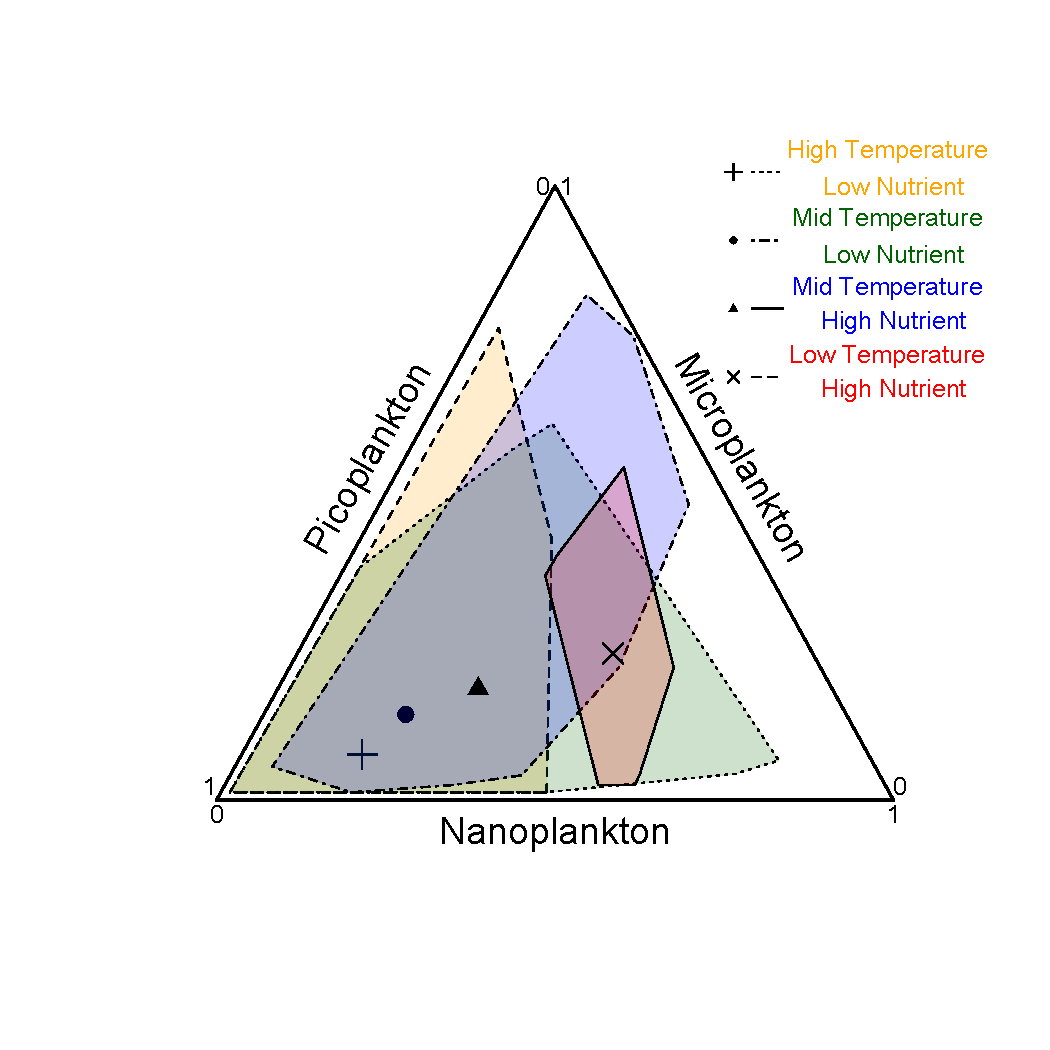
\includegraphics[trim = 12mm 15mm 10mm 15mm, clip, width=0.5\linewidth]{./Chp2-Pre/amt_clsEnvFINAL4-5.pdf}
\put(1,210){\textbf{b)}}
\put(-180,210){\textbf{a)}}
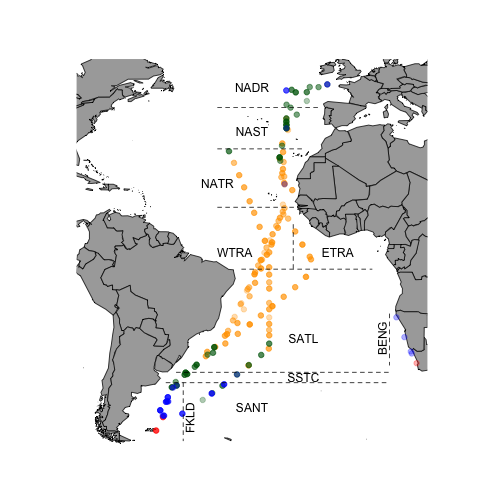
\includegraphics[trim = 20mm 20mm 20mm 20mm, clip, width=0.5\linewidth]{./Chp2-Pre/amt_mapClsEnv3.png}
\caption[Scheme]{\small {Caption comes here my friend""""""".}}
\label{clusters}
\end{figure}


\begin{figure}
\centering
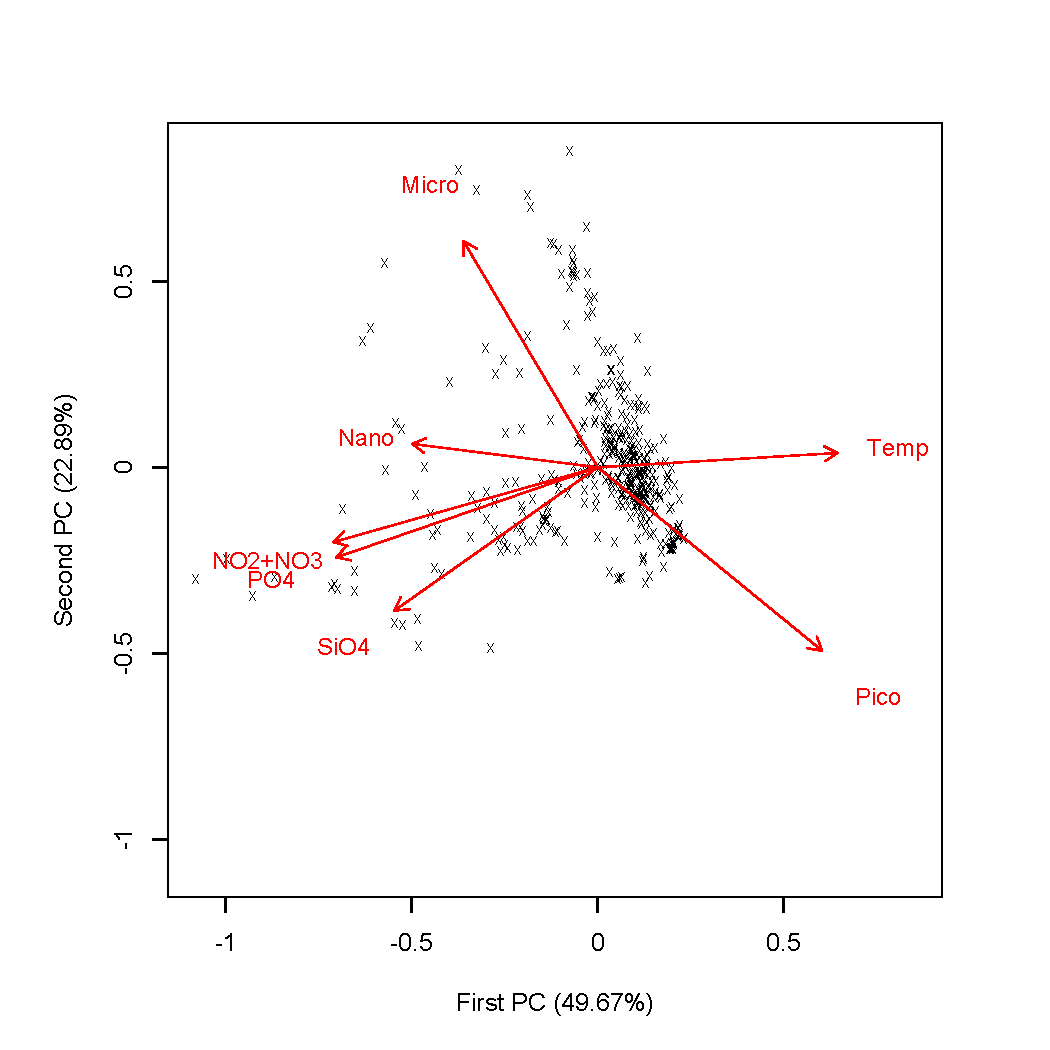
\includegraphics[trim = 0mm 0mm 0mm 0mm, clip, width=0.9\linewidth]{./Chp2-Pre/amt_PrinComp.pdf}
\caption[Scheme]{\small {Principal Component Analysis of environmental parameters and normalized phytoplankton size fractions.}}
\label{PrinComp}
\end{figure}

\begin{figure}
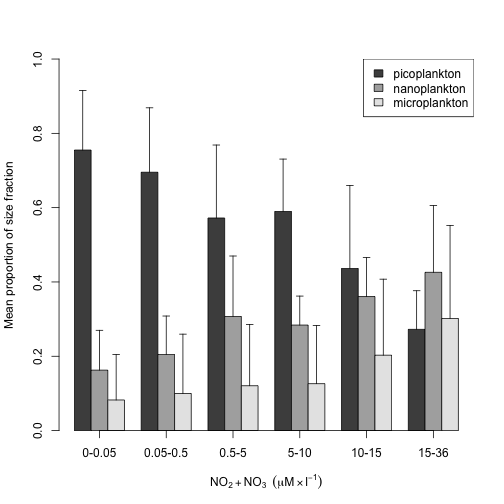
\includegraphics[trim = 0mm 0mm 0mm 15mm, clip, width=0.5\linewidth]{./Chp2-Pre/amt_NO3_bars2.png}
\put(-180,210){\textbf{a)}}
\put(1,210){\textbf{b)}}
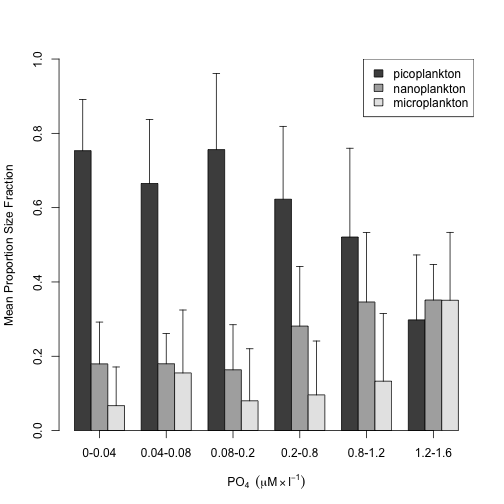
\includegraphics[trim = 0mm 0mm 0mm 15mm, clip, width=0.5\linewidth]{./Chp2-Pre/amt_PO4_bars2.png}
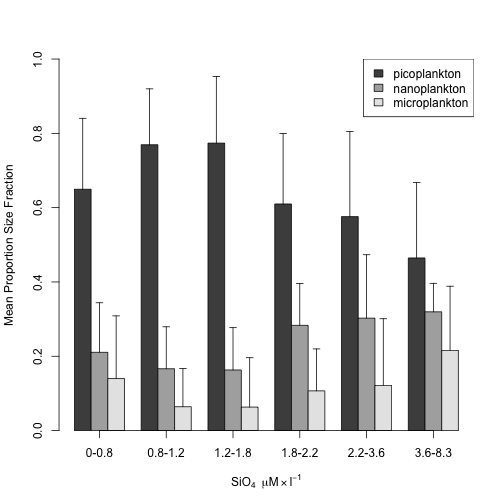
\includegraphics[trim = 0mm 0mm 0mm 15mm, clip, width=0.5\linewidth]{./Chp2-Pre/amt_SiO4_bars2.png}
\put(-180,210){\textbf{c)}}
\put(1,210){\textbf{d)}}
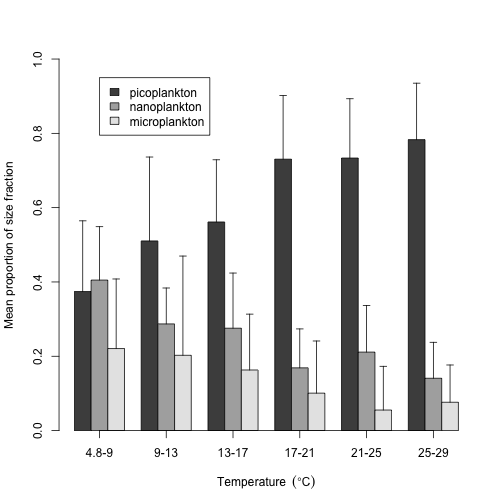
\includegraphics[trim = 0mm 0mm 0mm 15mm, clip, width=0.5\linewidth]{./Chp2-Pre/amt_Temp_bars2.png}
\caption[Scheme]{\small {Relative composition of picoplankton, nanoplankton and microplankton size fractions changing with concentrations of nitrate+nitrite (a), phosphate (b), and silicate (c) and with temperature (d). The bars represent mean values and the error bars indicate the standard deviation.}}
\label{response1}
\end{figure}

\begin{figure}
\centering
\includegraphics[trim = 0mm 0mm 0mm 15mm, clip, width=0.6\linewidth]{./Chp2-Pre/amt_zoo_bars2.png}
\caption[Scheme]{\small {Relative composition of picoplankton, nanoplankton and microplankton size fractions changing with copepod abundance. The bars represent mean values and the error bars indicate the standard deviation.}}
\label{response2}
\end{figure}

\begin{figure}
\centering
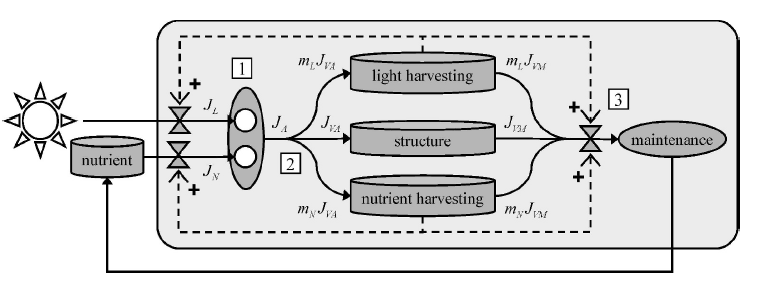
\includegraphics[trim = 0mm 0mm 0mm 0mm, clip, width=1\linewidth]{./Chp3-Further/Bruggeman-2007.png}
\caption[Scheme]{\small {Bruggeman and Kooijman model scheme. Taken from \citet{Bruggeman2007}}}
\label{Bruggeman}
\end{figure}


\begin{align*}
\frac{dP}{dt} & = \left[r(\bar{s})+\frac{1}{2}v\frac{\partial^{2} r(\bar{s})}{\partial s^{2}}\right]P \nonumber \\
& \nonumber \\
\frac{d\bar{s}}{dt} & = v\frac{\partial r(\bar{s})}{\partial s}\nonumber \\
&\nonumber \\
\frac{dv}{dt} & = v^{2}\frac{\partial^{2} r(\bar{s})}{\partial s^{2}}\nonumber\\
\end{align*}

The approach of defining a trade-off that relates size to the competitive ability for nutrient acquisition and resistance to predation \citep{Merico2009} leads to mechanistically capture bottom-up (nutrient availability and acquisition capabilities) versus top-down (avoid grazing) processes, major shaping forces of a phytoplankton community. The model will be tested against and constrained by the AMT observations on environmental data and community size structures in the Atlantic Ocean (chapter 2).  

\begin{figure}
\centering
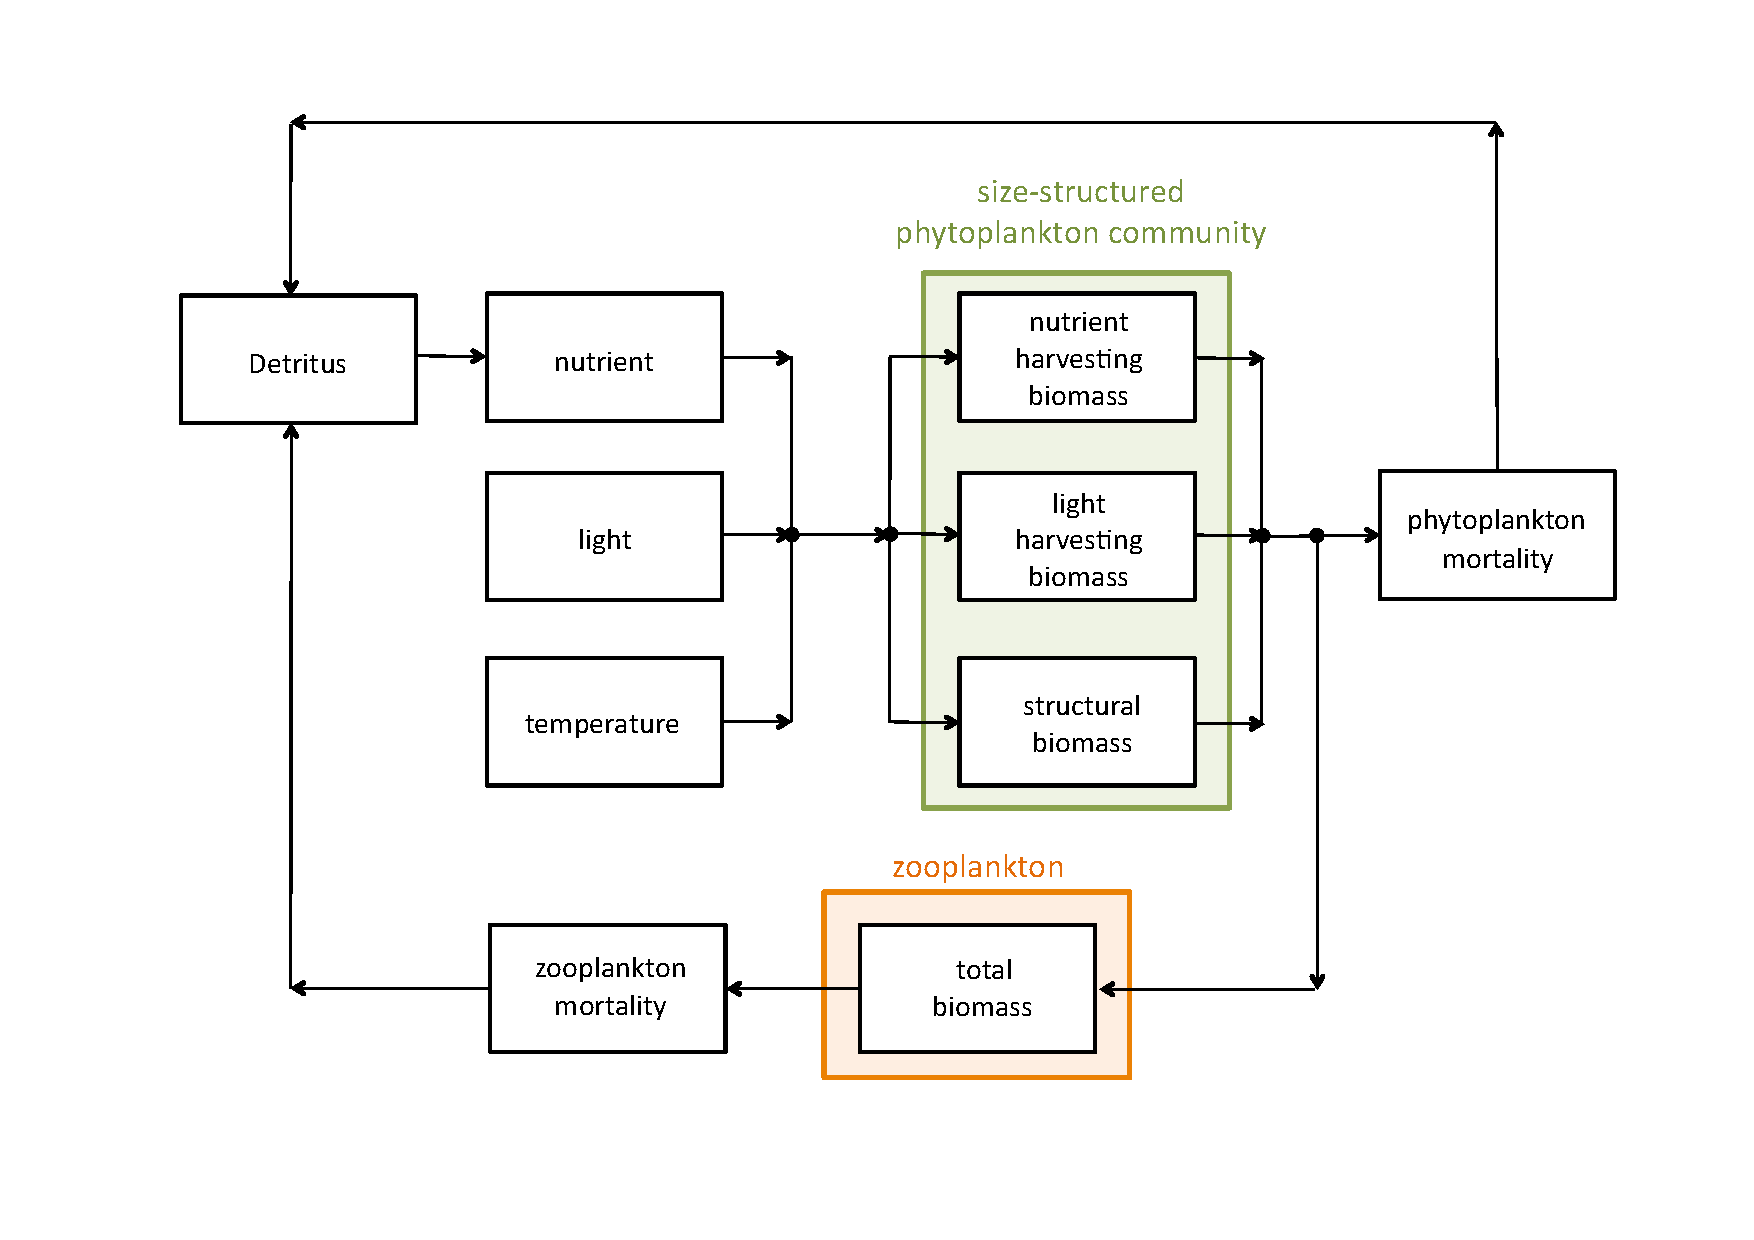
\includegraphics[trim = 15mm 50mm 15mm 25mm, clip, width=1\linewidth]{./Chp3-Further/model-scheme.pdf}
\caption[Scheme]{\small {Scheme of the proposed size-based model. In this model phytoplankton allocates energy (or biomass) to different pools such as nutrient and light harvesting biomasses and generic structural biomass. A certain fraction of the phytoplankton biomass flows into the zooplankton biomass and a remaining fraction is remineralized into the nutrient pool}}
\label{model}
\end{figure}

\begin{figure}
\centering
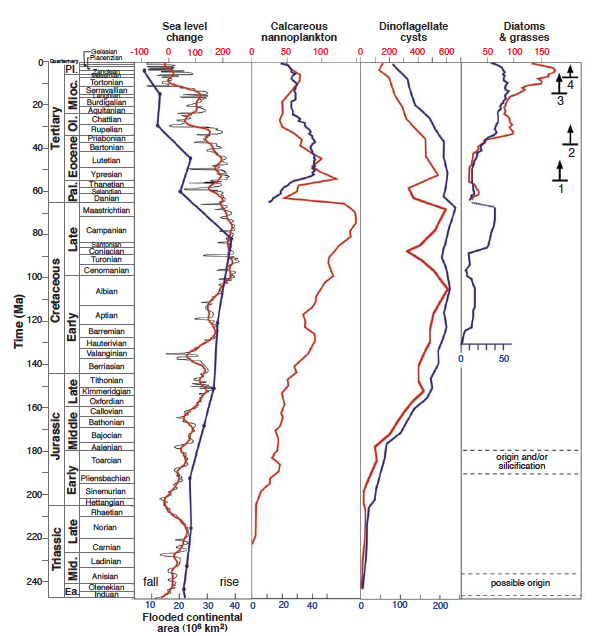
\includegraphics[trim = 0mm 0mm 0mm 0mm, clip, width=1\linewidth]{./Chp3-Further/Falkowski-2004.png}
\caption[Scheme]{\small {Comparison of major phytoplankton groups with sea-level change. The red line accounts for species diversities from published studies. The blue line accounts for the genus diversity compiled from public databases by the authors. Taken from \citet{Falkowski2004a}. }}
\label{Falkowski}
\end{figure}



%%%% TABLES %%%%

\begin{table}
\centering
\caption[Scheme]{\small {Mean values of environmental parameters for the different clusters: High temperature - Low nutrients (HTLN), Mid temperature - Low nutrients (MTLN), Mid temperature - High nutrients (MTHN and Low temperature - High nutrients (LTHN).}}
\label{tableclus}
\begin{tabular} {c c c c c}
cluster & NO$_2^-$ + NO$_3^-$ & PO$_4^{3-}$ & SiO$_4^{2-}$ & Temperature \\ \hline
HTLN & 0.150$\pm$0.575 & 0.064$\pm$0.078 & 1.097$\pm$0.575 & 25.299$\pm$2.000 \\
MTLN & 0.556$\pm$1.102 & 0.112$\pm$0.141 & 0.816$\pm$0.617 & 17.894$\pm$2.191 \\
MTHN & 9.027$\pm$3.593 & 0.799$\pm$0.373 & 2.423$\pm$1.375 & 11.925$\pm$2.797 \\
LTHN & 30.324$\pm$4.549 & 1.336$\pm$0.208 & 4.590$\pm$1.926 & 6.810$\pm$3.435 \\ \hline
\end{tabular}
\end{table}



\begin{table}
\centering
\caption[Scheme]{\small {Summary statistics for linear fittings of the three size fractions to each environmental variable.}}
\label{stats}
\begin{tabular} {c c c c c c c c c c }
& \multicolumn{3} {c} {Picoplankton} & \multicolumn{3} {c} {Nanoplankton} & \multicolumn{3} {c} {Microplankton} \\
& slope & p-value & $r^2$ & slope & p-value & $r^2$ & slope & p-value & $r^2$ \\ \hline
NO$_2^-$ + NO$_3^-$ &-0.090 &0.002 & 0.908 &0.050 &0.001 & 0.921 &0.040 &0.010 &0.792 \\
PO$_4^{3-}$ &-0.0812 &0.021 &0.711 &0.042 &0.012 &0.777 &0.039 &0.125 &0.354 \\
SiO$_4^{2-}$ &-0.047 &0.085 &0.455 &0.030 &0.044 &0.597 &0.016 &0.247 &0.142 \\ 
Temperature &0.082 &0.001 &0.914 &-0.047 &0.008 &0.812 &-0.035 &0.003 &0.885 \\
Copepods &-0.063 &0.064 &0.520 &0.068 &0.051 &0.567 &-0.004 &0.788 &-0.222\\ \hline
\end{tabular}
\end{table}

%%%% typical text %%%%

Smaller phytoplankton cell sizes have a competitive advantage over larger phytoplankton under low nutrient, low light and low grazing pressure \citep{Litchman2008, Litchman2010}. From our regression analyses (Figures \ref{response1} and \ref{response2}) we inferred a strong control of NO$_3^-$+NO$_2^-$ and temperature on all three size fractions. Pico- and nanoplankton size fractions, however, appeared more sensitive to changes in PO$_4^{3-}$, SiO$_4^{2-}$ and copepod abundance. We propose that these effects are caused by a trade-off between resource acquisition and predation pressure, although with the caveat represented by the paucity of the zooplankton data and by the qualitative value we attribute to zooplankton abundance as an indication of grazing pressure. There are a number of important physiological and ecological processes that strongly depend on phytoplankton cell size \citep{Kiorboe1993, Cermeno2008a, Finkel2009a}, including metabolic rates, maximum nutrient uptake rate, nutrient diffusion, light absorption, sinking velocity, trophic interactions and even diversity within taxa, which is often a log-normal distribution of body size. Our results are therefore consistent with this general "size rule" \citep{Finkel2009a}. To our knowledge it is the first time that this feature is observed in data extending across an entire ocean basin and irrespective of temporal changes.